\documentclass{article}
\usepackage{cmap}
\usepackage[T2A]{fontenc}
\usepackage[utf8]{inputenc}
\usepackage[english,russian]{babel}
\usepackage{setspace}
\usepackage{geometry}
\usepackage{graphicx}
\usepackage{amsfonts}
\usepackage{amsmath}
\graphicspath{{graphicslab7/}}
\DeclareGraphicsExtensions{.pdf, .png, .jpg, .fig}
\geometry{top=2cm}
\geometry{bottom=2cm}
\geometry{left=2cm} % отступ справа
\geometry{right=2cm} % отступ слева

\begin{document}
	\begin{center}
		\hfill \break
		\begin{center}
			\huge{Санкт-Петербургский политехнический университет\\
				Высшая школа прикладной математики\\
				и вычислительной физики, ФизМех} 
		\end{center}
		\hfill \break
		\hfill \break
		\hfill \break
		\hfill \break
		\hfill \break
		\huge{Направление подготовки\\
			«Прикладная математика и информатика»}\\
		\hfill \break
		\hfill \break
		\hfill \break
		\hfill \break
		\hfill \break
		\hfill \break
		\fontsize{14pt}{14pt}\selectfont
		Отчет по лабораторной работе №7\\
		«Численнные методы решения краевых задач для обыкновенных дифференциальных уравнений»\\
		\hfill \break
		\hfill \break
		\hfill \break
		\hfill \break
		\hfill \break
	\end{center}
	\hfill \break
	\hfill \break
	\fontsize{12pt}{12pt}\selectfont
	\begin{tabular}{cccc}
		\hspace{1cm}Выполнил студент гр. 5030102/00003 & {\hspace{3cm}} & & Петрошенко А.В. \\\\
		\hspace{-3cm}Преподаватель: &{\hspace{1cm}}& & {\hspace{1cm}} Курц В.В. \\\\
	\end{tabular}\\
	\hfill \break
	\hfill \break
	\hfill \break
	\hfill \break
	\hfill \break
	\hfill \break
	\begin{center} Санкт-Петербург\\ 
		2021\\
	\end{center}
	\thispagestyle{empty}
	\newpage
	\begin{center} \textbf{Формулировка задачи и ее формализация}\end{center}
	Дано ОДУ 2-го порядка с переменными коэффициентами:
	\begin{equation}
		p(x)y'' + q(x)y' + r(x) = f(x)
	\end{equation}
	$p(x), q(x), r(x), f(x) \in C([a,b])$
	Дифференциальный оператор $\displaystyle L = p\frac{d^2}{dx^2} + q\frac{d}{dx} + r$. Тогда (1) $\Leftrightarrow L(y) = f$\\
	Общий вид граничных условий:
	\begin{equation}
		\begin{cases}
			\alpha_0y(a) + \alpha_1y'(a) = A\\
			\beta_0y(b) + \beta_1y'(b) = B
		\end{cases}
	\end{equation}
	$\alpha_0^2+\alpha_1^2 \neq 0$, $\beta_0^2+\beta_1^2 \neq 0$\\
	И дополнительное условие $\beta_1 \neq 0$
	\underline{постановка задачи:}\\
	Необходимо решить краевую задачу на отрезке $[0,1]$ вида:
	\begin{equation}
		\begin{cases}
			(e^x + 1)y'' - y' - e^xy = e^x\\
			-y'(a) = -1\\
			y(b) + y'(b) = 2e - 1
		\end{cases}
	\end{equation}
	т.е. $\alpha_0 = 1$, $\alpha_1 = -1$, $\beta_0 = 1$, $\beta_1 = 1$\\
	Нужно вычислить точное решение $y^*(x) = e^x - 1$
	\begin{center} \textbf{Алгоритм метода и условия его применимости}\end{center}
	Заменим производные конечными разностями:
	\begin{equation}
		\frac{dy}{dx} = \frac{y_{i+1} - y_{i-1}}{2h}
	\end{equation}
	Тогда вторая производная будет иметь вид:
	\begin{equation}
		\frac{d^2y}{dx^2} = \frac{y_{i+1} - 2y_i + y_{i-1}}{h^2}	
	\end{equation}
	Теперь вместо ДУ будем решать СЛАУ:
	\begin{equation}
		\begin{cases}
			\displaystyle \alpha_0y_0 + \alpha_1\frac{-3y_0 + 4y_1 - y_2}{2h} = A\\
			\displaystyle p_k\frac{y_{k+1} - 2y_k + y_{k-1}}{h^2} + q_k\frac{y_{k+1} - y_{k-1}}{2h} + r_ky_k = f_k\\
			\displaystyle \alpha_0y_0 + \alpha_1\frac{3y_n - 4y_{n-1} + y_{n-2}}{2h} = B
		\end{cases}
	\end{equation}
	Данная матрица практически трехдиагональная, за исключением первой и последней строчки. Приведем ее к трехдигональной вычитанием соседних строк и решим ее, например, алгоритмом прогонки. Получим вектор $Y$, который и будет решением исходного ОДУ.
	\underline{Условия применимости:}
	\begin{enumerate}
		\item $\alpha_0^2+\alpha_1^2 \neq 0$, $\beta_0^2+\beta_1^2 \neq 0$, $\beta_1 \neq 0$
		\item По теореме должны выполнятся 3 условия:
		$$
		\begin{cases}
			p(x) \geq 0\\
			p(x) \geq \frac{h}{2}|q(x)|\\
			r(x) \leq 0
		\end{cases}
		$$
		\item Так как мы будем решать трехдиагональную матрицу, то она должна обладать диагональным преобладанием для устойчивости метода прогонки 
	\end{enumerate} 
	\begin{center} \textbf{Предварительный анализ задачи}\end{center}
	\begin{enumerate}
		\item Из выбора коэффициентов данные условия выполнены по построению
		\item Все 3 условия теоремы выполнены:
		$$
		\begin{cases}
			e^x + 1 \geq 0\\
			e^x  + 1 \geq \frac{h}{2}|-1|\\
			-e^x \leq 0
		\end{cases}
		$$
		\item Промежуточные строки матрицы(не первая и не последняя) обладают диагональным преобладанием: $\displaystyle e^{x_i}h^2 + 2(e^{x_i} + 1) \geq (-(e^{x_i} + 1) - \frac{h}{2}) + (\frac{h}{2} - (e^{x_i} + 1)) = -2(e^{x_i} + 1)$.\\ 
		Т.к. при приведении к трехдиагональной матрицы мы из не дигонального элемента вычитали диагональный и наоборот, т.е. из большего меньшее и из меньшего большее, то нам достаточно проверить исходные коэффициенты, чтобы первая и последняя строки тоже обладали диагональным преобладанием:
		$\displaystyle \alpha_0h - \frac{3}{2}\alpha_1 = h + \frac{3}{2} \geq -2 = 2\alpha_1$
	\end{enumerate}
	\begin{center} \textbf{Тестовый пример для задач малой размерности}\end{center}
	Протестируем метод, разбив данный отрезок $[0,1]$ на 5 частей. Тогда $k=5$, $\displaystyle h = \frac{b-a}{k} = 0.2$\\
	Точное решение: $y^*(x) = e^x - 1$
	\begin{center}
		\begin{tabular}{|c|c|c|c|c|c|c|}
			\hline
			x & 0 & 0.2 & 0.4 & 0.6 & 0.8 & 1\\
			\hline
			y & 0 & 0.221 & 0.492 & 0.822 & 1.225 & 1.718\\
			\hline
		\end{tabular}
	\end{center}
	Построим матрицу по формулам (6) и сразу преобразуем ее в трехдигональную:

	\begin{equation}
		A = \left(
		\begin{array}{cccccc}
			1.153 & -0.941 & 0 & 0 & 0 & 0\\
			-2.321 & 4.492 & -2.121 & 0 & 0 & 0\\
			0 & -2.592 & 5.043 & -2.392 & 0 & 0\\
			0 & 0 & -2.922 & 5.717 & -2.722 & 0\\
			0 & 0 & 0 & -3.325 & 6.540 & -3.125\\
			0 & 0 & 0 & 0 & -1.017 & 1.230
		\end{array}
		\right)
	\end{equation}
	Вектор свободных членов $F$ будет выглядеть так:
	\begin{equation}
		F = (-0.211, -0.049, -0.060, -0.073, -0.090, 0.874)
	\end{equation}
	Теперь решаем эту СЛАУ методом прогонки и получаем вектор $Y$:
	\begin{equation}
		Y = (-0.003, 0.221, 0.494, 0.827, 1.234, 1.730)
	\end{equation}
	Как видно значения практически совпадают, график точного и численного решения для 5 частей представлен ниже.
	\begin{center} \textbf{Контрольные тесты}\end{center}
	\begin{enumerate}
		\item Разобъем отрезок $[0,1]$ на 5 частей, решим ДУ и посмотрим на графики точного и численного решения, а так же на график ошибки.
		\item Будем разбивать наш отрезок на части (от 10 до 500 с шагом 1) каждый раз решая ДУ и вычисляя норму вектора погрешности.
		\item Разобъем отрезок $[0,1]$ на 10 частей и будем вносить в граничные условия возмущения различного порядка(от $10^{-10}$ до 1) относительно порядка значения условия
	\end{enumerate}
	\begin{center} \textbf{Модульная структура программы}\end{center}
	\verb|double p(double x)|\\
	\verb|double q(double x)|\\
	\verb|double r(double x)|\\
	\verb|double f(double x)|\\
	-Функции переменных коэффициентов.\\
	\verb|vector<vector<double>> CreateMatrix(double a, double b, int n, double alpha0,|\\ \verb|double alpha1, double beta0, double beta1, double A, double B);|\\
	-Функция задания матрицы.\\
	\verb|vector<double> ThomasAlgorithm(vector<double> w0, vector<double> w1,|\\ \verb|vector<double> w2, vector<double> F);|\\
	-Алгоритм прогонки, возвращающий вектор $Y$.
	\begin{center} \textbf{Численный анализ}\end{center}
	$\triangleright$ \underline{Точное и численное решение:}\
	\begin{center} \includegraphics[scale = 0.6]{решения} \end{center}
	Оба графика накладываются друг на друга, что показывает, что решения практически совпадают.\\
	$\triangleright$ \underline{Ошибка численного решения:}
	\begin{center} 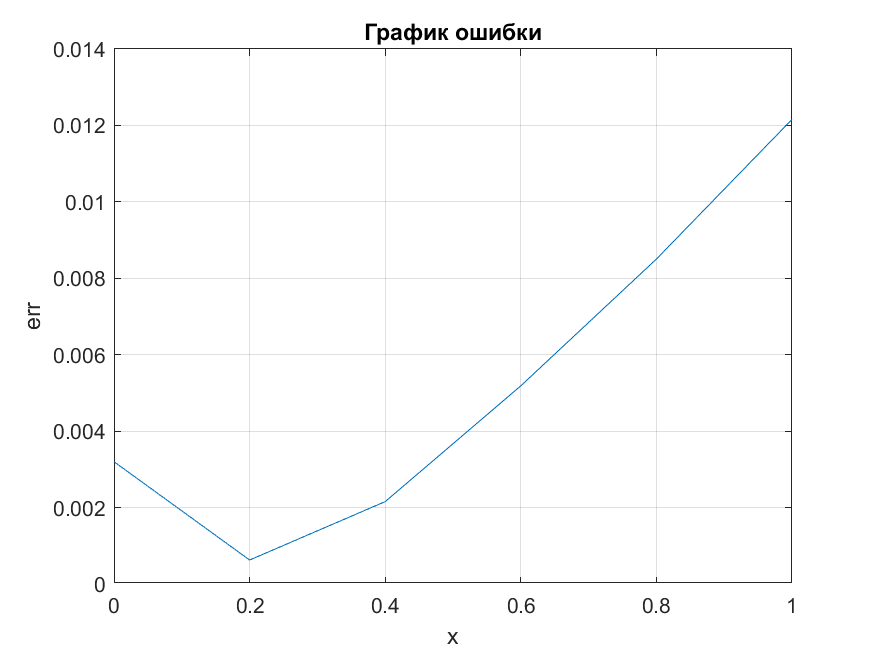
\includegraphics[scale = 0.6]{ошибка} \end{center}
	В граничных точках ошибка ненулевая, т.к. в условии присутствовала производная. Значит минимум ошибки будет где-то между границами отрезка, так оно и есть.\\
	$\triangleright$ \underline{Погрешности:}
	\begin{center} 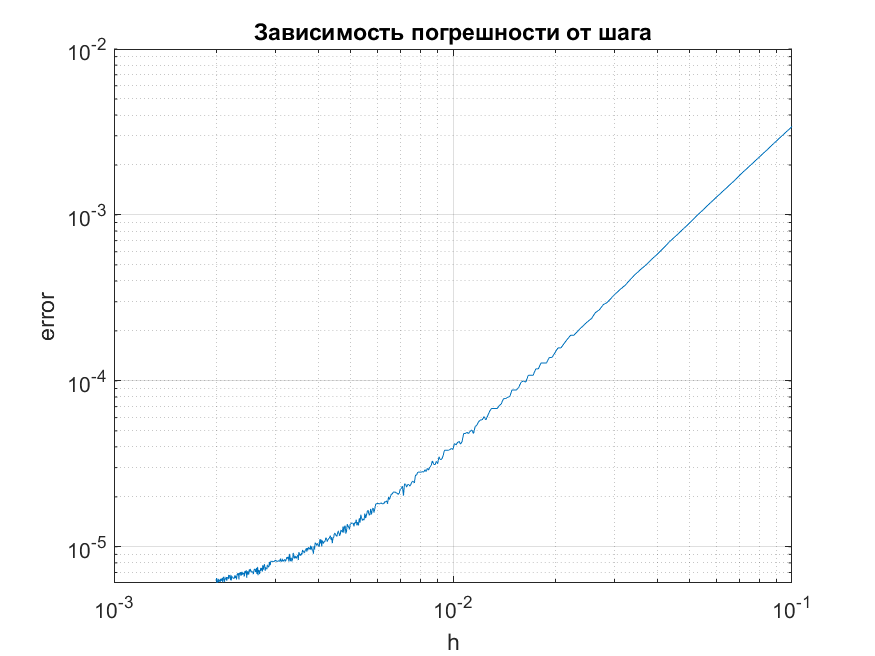
\includegraphics[scale = 0.6]{погрешность} \end{center}
	Порядок погрешности совпадает с порядком метода. На малых $h$ происходят колебания, которые вызвана вычислительной погрешностью алгоритма прогонки, поскольку матрица становится большой.\\
	$\triangleright$ \underline{Возмущение:}
	\begin{center} 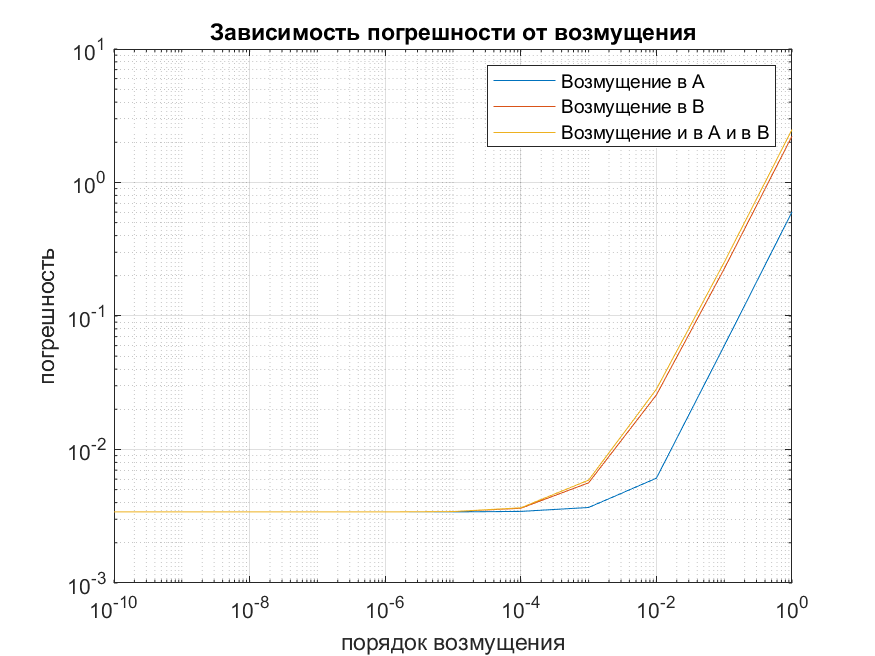
\includegraphics[scale = 0.6]{возмущение} \end{center}
	Мы рассмотрели 3 возмущения: 2 только в одном граничном условии и 1 в обоих. При малых возмущениях погрешность не меняется, но начиная с $10^{-5}$ они отклоняются, . Так же можно рассмотреть противоположные возмущения для каждого случая, но на картину это повлияет не сильно
	\begin{center} \textbf{Общие выводы}\end{center}
	В данной лабораторной работе мы научились численно решать ОДУ 2-го порядка на заданном промежутке с помощью метода конечных разностей 2-го порядка с ненулевым коэффициентом $\beta_1$. Реализация метода довольно трудная, т.к. нужно построить матрицу, привести ее к трехдиагональной и решить. К тому же метод требует довольно много вычислений, что влияет на конечную погрешность.
\end{document}